\documentclass[12pt]{article}

%Packages________________
\usepackage[normalem]{ulem}
\usepackage[dvipsnames]{xcolor}
\usepackage{cancel}
\usepackage{parskip}
\usepackage[font=small,labelfont=bf]{caption}
\usepackage{subcaption}
\usepackage[Spanish,es-tabla,es-noshorthands]{babel}
\usepackage{newtxtext}
\usepackage[varvw]{newtxmath}
\usepackage{booktabs, colortbl, bigstrut, multirow, multicol}
\usepackage{url}
\usepackage{pgfplots}
\usepackage{graphicx}
\usepackage{amsmath}
\usepackage{tabularx}
\usepackage{floatrow}
\usepackage{float}
\usepackage{cancel}
\usepackage[spanish]{cleveref}
\usepackage{tikz}
\usetikzlibrary{arrows.meta,shapes.geometric,positioning,calc}
\crefname{table}{tabla}{tablas}
\usepackage{wrapfig}
\usepackage{adjustbox}
\usepackage{geometry}
\usepackage{lipsum}
\usepackage{fancybox}
\usepackage[T1]{fontenc}
\geometry{
	left=3cm,
	right=3cm
}

\usepackage[
    backend=biber,
	citestyle=verbose-ibid,
    bibstyle=authoryear-icomp,
    natbib=true,
    url=true, 
    doi=true,
    eprint=false
]{biblatex}

\addbibresource{ref.bib}

%Commands________________
\newcommand\hcancel[2][black]{\setbox0=\hbox{$#2$}%strikeout
\rlap{\raisebox{.45\ht0}{\textcolor{#1}{\rule{\wd0}{1pt}}}}#2} 

\renewcommand\theequation{\Alph{equation}}

\def\mydate{\leavevmode\hbox{\twodigits\day/\twodigits\month/\the\year}}
\def\twodigits#1{\ifnum#1<10 0\fi\the#1}

\newcommand\runinsec{\@startsection {section}{1}{\z@}%
                                   {3.5ex \@plus 1ex \@minus .2ex}%
                                   {-1em}%
                                   {\normalfont\Large\bfseries}}
\newcommand\aftersec[1]{\begingroup\normalfont\footnotesize #1\endgroup%
                        \par\nobreak\vspace*{2.3ex}\noindent\ignorespaces}

%\renewcommand\thesubsection{\alph{subsection}}

% \input{colorbox.txt}

\usepackage{listings}
\lstset{%
basicstyle=\ttfamily,
breaklines = true,
backgroundcolor=\color{mygray},
}
\definecolor{mygray}{rgb}{0.8,0.8,0.8}
\newcommand{\code}[1]{\colorbox{mygray}{\lstinline|#1|}}

\usepackage{dirtree}

\def\mydate{\leavevmode\hbox{\twodigits\day/\twodigits\month/\the\year}}
\def\twodigits#1{\ifnum#1<10 0\fi\the#1}

%Titlepage_________________
\title{\vspace{-1.8cm} Prueba de Evaluación Contínua}
\author{Álvaro Jerónimo Sánchez}
\date{\vspace{-0.6cm}\small\mydate}

%Document_____________
\begin{document}
\maketitle
\setcounter{section}{0}
\renewcommand{\tablename}{Tabla}

\textbf{ESPECIFICACIONES DE LA PRUEBA}

No se han empleado librerías que no sean estándar, y los archivos de cada ejercicio se encuentran en el mismo directorio de este \textit{PDF} con los nombres ``\textit{ejercicio\_n}'' con su extensión correspondiente (\textit{.c}, \textit{.m}). No se han empleados argumentos de línea de comandos ni opciones de compilación, todos los parámetros están dentro del código como variables. No se crearán directorios adicionales a la hora de generar los archivos de datos para evitar confusiones, todos los arhcivos estarán dentro de este mismo directorio. Este documento ha sido generado con \LaTeX , si fuese necesario, proporcionaré el archivo \textit{.tex} y todas las figuras adjuntas a petición vuestra.

En el directorio se encuentran los siguientes archivos:
\dirtree{%
.1 JERONIMO\_SANCHEZ\_ALVARO\_PEC.zip.
.2 ejercicio\_1.c.
.2 ejercicio\_2.m.
.2 ejercicio\_3.m.
.2 memoria\_resultados.pdf.
}


\section{Simulación numérica en C}

\subsection{Discretización del sistema e implementación del algoritmo}

Los mecanismos de \textit{reacción-difusión}, propuestos por Alan Turing, explican cómo los patrones presentes en diversos animales son resultado de reacciones entre dos o más sustancias químicas (activador-inhibidor) con pequeñas perturbaciones que acaban causando estructuras periódicas. Este ejercicio es la parte principal de la simulación que generará los datos a partir de los parámetros introducidos. Se resolverán las ecuaciones de dicho modelo creando una red $L \times L$, introduciendo perturbaciones y calculando el \textit{laplaciano} en cada punto discreto. Se ha decidido definir funciones para la mayoría de operaciones necesarias y luego llamarlas en \code{int main()}.

Se ha inicializado las matrices en el estado homogéneo con los parámetros iniciales dados:
\begin{gather*}
	L=100,\; Du=1,\; Dv=10,\; a=0.1,\; b=0.9,\; dt=0.01s,\; T=200s\\
	U_{0(L\times L)}=\left(
	\begin{array}{cc}
		u_0 & \cdots\\
		\vdots & \ddots
	\end{array}
	\right) \; ; \;
	V_{0(L\times L)} = \left(
	\begin{array}{cc}
		v_0 & \cdots\\
		\vdots & \ddots
	\end{array}
	\right)\\
	\text{siendo: } u_0=a+b ,\; v_0=\frac{b}{(a+b)^2}
\end{gather*}

 Tras inicializar las matrices, se ha añadido un ruido gaussiano aleatorio con una función \code{gauss} aplicando la transformada de Box-Muller a cada punto de la matriz, cuya fórmula es:
\begin{gather*}
	z = \sqrt{-2\ln u_1}\, \cos(2\pi u_2)
\end{gather*}
Siendo $z$ la perturbación generada, y $u_1,\, u_2$ son números aleatorios entre 0 y 1.

Posteriormente, en la función \code{timestep}, se crean dos nuevas matrices de las mismas dimensiones para ir actualizando con cada paso. Es necesario calcular los valores de $v$ para sustituir en la fórmula de $u$, aunque la matriz a estudiar en la que se observa el patrón es la $u$. En cada paso temporal, se calcula el cálculo del tiempo (empleando los datos del paso anterior) en cada punto de la matriz \textit{u} con las fórmulas:
\begin{gather*}
	u_{i,j}^{n+1} = u_{i,j}^n + dt \left( D_u \nabla^2 u_{i,j}^n + a - u_{i,j}^n + (u_{i,j}^n)^2 v_{i,j}^n \right) \\
	v_{i,j}^{n+1} = v_{i,j}^n + dt \left( D_v \nabla^2 v_{i,j}^n + b - (u_{i,j}^n)^2 v_{i,j}^n \right)
\end{gather*}

Y siendo el laplaciano:
\begin{gather*}
	\nabla^2 u_{i,j} = u_{i+1,j}+u_{i-1,j}+u_{i,j+1}+u_{i,j-1}-4u_{i,j}
\end{gather*}

Tras recorrer los pasos determinados y escribirlos en un archivo con una función \code{filesave}, se repite hasta generar los 10 documentos \textit{.dat}, del 0 al 9, correspondientes a 20 000 pasos temporales.

Cabe mencionar que se han aplicado las condiciones de contorno con funciones \code{if}, igualando los vecinos que ``se salen'' por un lado (``arriba, abajo, izquierda, derecha'') al primero del lado opuesto. De esta manera no hay comportamientos indeterminados en los bordes.

\subsection{Amplitud de la perturbación}

Para hallar la amplitud, se calcula el promedio de $(u-u_0)^2$ para cada paso, siendo $u$ el valor de cada punto de la red en dicho paso (que se graba en la misma función \code{timestep}) y $u_0$ el valor fijo inicial sin las perturbaciones $(a+b)$. Se usa esto para la fórmula:
\begin{gather*}
	A(t) = \sqrt{\langle(u-u_0)^2\rangle}
\end{gather*}

El resultado se guarda junto al índice del paso del tiempo con su propia función \code{ampsave}. Además, se crea un archivo \textit{time.dat} con los índices de cada paso temporal.

\section{Análisis de resultados en MATLAB}

\subsection{Visualización del patrón}

\begin{wrapfigure}{r}{0.6\textwidth}
\centering
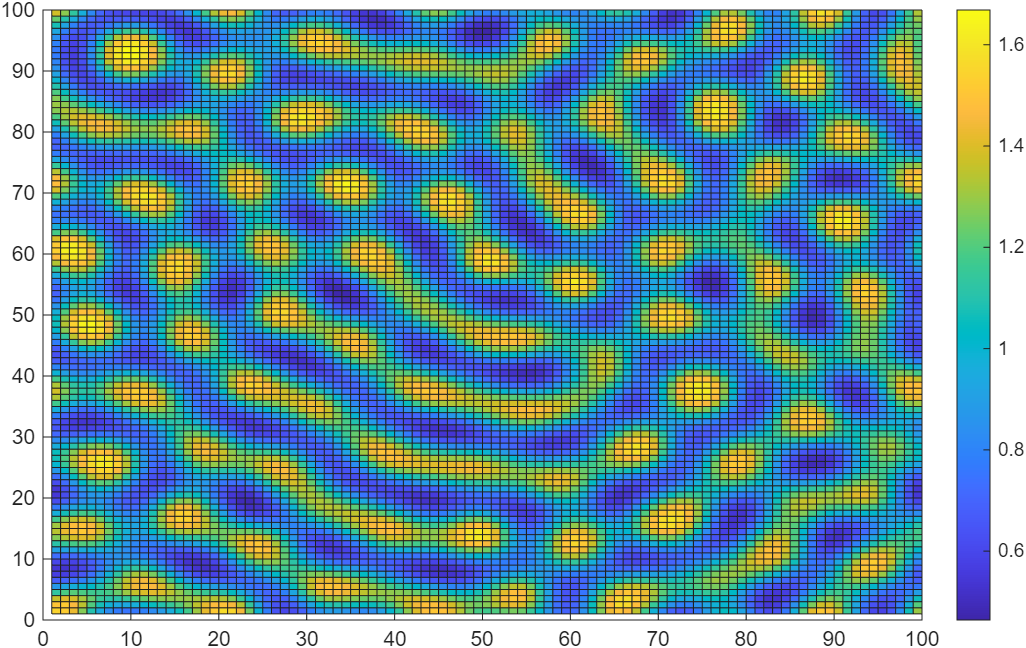
\includegraphics[width=0.95\columnwidth]{final.png}
\captionof{figure}{Estado final del patrón generado en la matriz $u$.}
\label{fig:pat}
\end{wrapfigure}

En \textit{MATLAB} podremos analizar los resultados obtenidos en la simulación y observar la evolución del patrón generado. Se ha empleado la función \code{readmatrix} para leer los contenidos de los archivos \textit{.dat} generados con C. Posteriormente, se ha buscado el máximo y mínimo global para usarlos en la escala de color. Se ha usado un bucle que repite los diez pasos de la animación desde principio hasta fin.

El patrón final resultante tiene un aspecto laberíntico, con curvas cuyas tangentes aparentan ser prácticamente paralelas entre ellas en sus caminos, como si girasen alrededor de un mismo radio. Presenta focos circulares con perturbaciones más intensas, y se puede ver cómo las condiciones de contorno se cumplen: si situamos la misma figura duplicada en cualquiera de los bordes, ambas ``encajan''. La apariencia de este patrón es la esperada de un patrón de Turing.

\subsection{Evolución temporal de la perturbación}

\begin{figure}[h]
  \begin{floatrow}
    \ffigbox{
\includegraphics[width=0.7\columnwidth]{graph.png}}
    {\caption{Sección exponencial y ajuste lineal de la amplitud de la perturbación en escala logarítmica con el tiempo.}
    \label{fig:gr}}
    \ffigbox{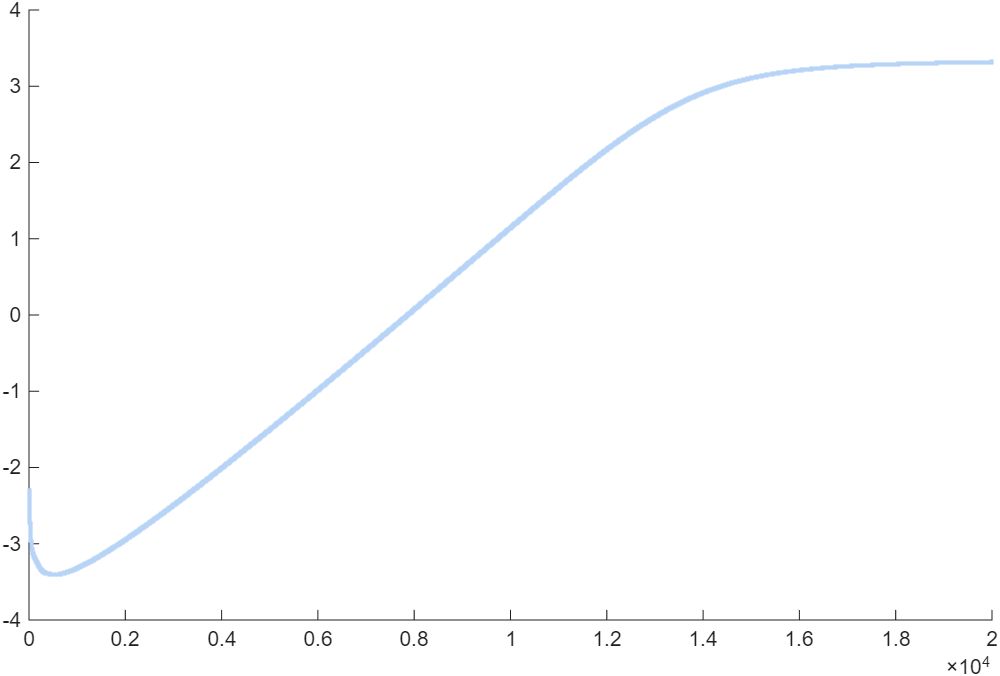
\includegraphics[width=0.7\columnwidth]{graph_complete.png}}
    {\caption{Gráfica completa de la evolución de la amplitud de la perturbación en escala logarítmica con el tiempo.}
    \label{fig:grc}}
  \end{floatrow}
\end{figure}


La evolución de la amplitud de la perturbación se ha representado en una figura separada a la del patrón. Se ha situado este código antes del bucle de la animación para que pueda generarse la gráfica de la amplitud de la perturbación antes del \code{while} infinito.

Al representar $A(t)$ en escala logarítmica, una recta diagonal representa crecimiento exponencial, por lo que esa será la sección que escojamos. Se ha hecho un ajuste lineal (línea roja), cuya solución se ha imprimido en pantalla, y a la vez se han representado los datos medidos con una gráfica \code{scatter} de puntos azules.

En la gráfica completa (\cref{fig:grc}), inicialmente, hay una caída vertical hasta que el sistema se estabiliza y empieza a mostrar un crecimiento exponencial. Desde $t=1.4\cdot 10^4$ la amplitud decrece hasta ser horizontal, ya que aquí está llegando a su estado final en el que no va a crecer o cambiar más. Esto encaja con lo esperado para el sistema de activador-inhibidor, ya que se observa que a partir de unas pequeñas perturbaciones en un sistema homogéneo, el sistema genera patrones periódicos que crecen hasta estabilizarse.

\section{Análisis de estabilidad lineal}

\subsection{Autovalores del Jacobiano}

Se ha inicializado la matriz con los valores iniciales sustituyendo los parámetros $u_0=a+b$ y $v_0=\frac{b}{(a+b)^2}$ sabiendo que el Jacobiano es:
\begin{gather*}
	J = \left(
	\begin{array}{cc}
		-1+2u_0v_0 & u_0^2\\
		-2u_0v_0 & -u_0^2
	\end{array}
	\right)
\end{gather*}
Se han hallado sus autovalores con la función \code{eig()}. Se ha hallado que ambos autovalores tienen parte real negativa $\boxed{-0.1000}$. El tipo de punto fijo es un \textbf{foco}, ya que los autovalores son complejos conjugados, y es \textbf{asintóticamente estable} ya que ambas partes reales de los autovalores son negativas:
\begin{gather*}
	\lambda_1 = -0.1000 + 0.9950i\, ; \; \lambda_2 = -0.1000 - 0.9950i
\end{gather*}

\subsection{Barrido en número de onda}

\begin{wrapfigure}[15]{r}{0.6\textwidth}
\centering
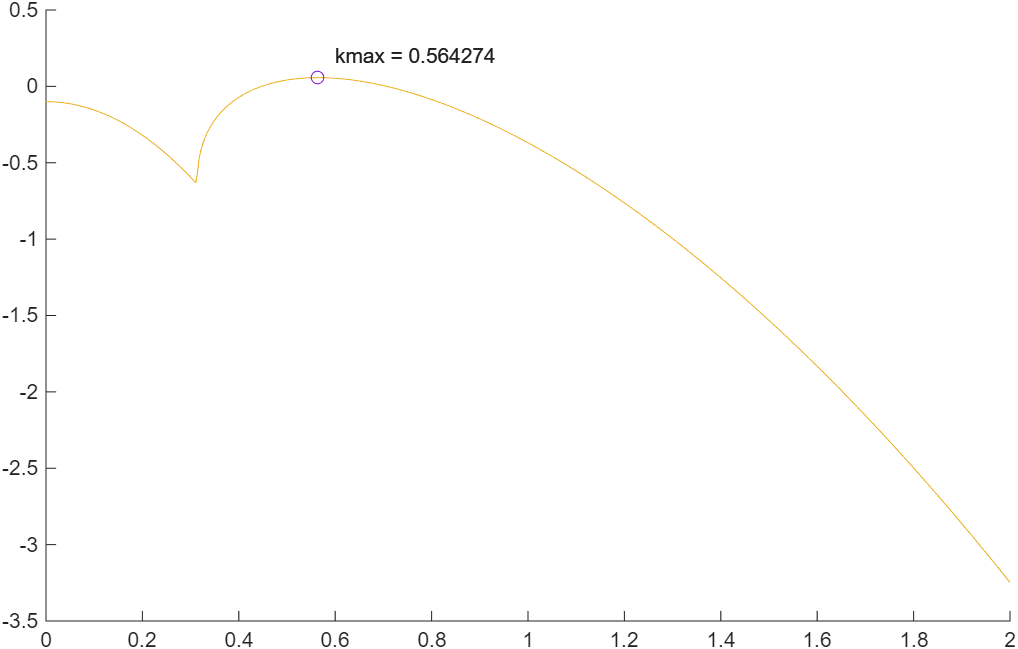
\includegraphics[width=0.95\columnwidth]{barrido.png}
\label{fig:barr}
\caption{Relación de dispersión: parte real del autovalor dominante en función de $k$. Se ha marcado $k_{máx}$ con un círculo magenta.}
\end{wrapfigure}

Usando el Jacobiano planteado anteriormente, podemos hallar la evolución de las perturbaciones con la matriz:
\begin{gather*}
	M(k) = J-\left(
	\begin{array}{cc}
		D_uk^2 & 0\\
		0 & D_vk^2
	\end{array}
	\right)
\end{gather*}

Se quiere hallar el valor de $k$ para el cual $M(k)$ es máximo para un rango $[0,2]$. Se ha decidido analizar 600 puntos de dicho intervalo. Se ha representado 
la parte real del autovalor dominante en función de $k$ (relación de dispersión), y se ha elegido el valor de $k$ máximo para el que la función sea máxima. Se ha marcado el punto en la gráfica y se ha mostrado su valor en pantalla.

\vspace{1cm}
\textit{\textbf{Nota:} Se ha buscado la $k_{máx}$ empleando la función \code{find()} de MATLAB, ya que en el guión parece especificarse que hay que hallar el valor máximo de ésta. Realmente sólo sería necesario en el caso de que haya dos valores de $k$ con un mismo máximo, en cuyo caso se elegiría la $k$ mayor entre las dos.}
%_________________________________________

%\nocite{*}
%\printbibliography

\end{document}